\documentclass{article}
\usepackage{graphicx}
\usepackage{geometry}
\usepackage{subcaption}
\usepackage{amsmath, amssymb}
\geometry{tmargin=3cm, lmargin=3cm, rmargin=2cm, bmargin=2cm}

\begin{document}
\section{Grid graph}
A comprehensive performance evaluation of our spectral graph topology algorithm was
performed considering a grid graph model with 64 nodes $\mathcal{G}^{(64)}_{\mathsf{grid}}$.
The edges of the grid graph are sampled from $\mathsf{Uniform}(0.1, 3)$.
Then we estimate the Laplacian matrix based on $T$ samples from $\mathcal{N}(\mathbf{0}, \mathbf{L}_{\mathsf{grid}}^{\dagger})$
and compute the relative error and the F-score. We perform that 100 times for a fixed number $T$ and we average out the relative errors
and F-scores.

For the values of $T$ such that $T / N > 1$, we fix $\beta = 4$. Otherwise, we start with $\beta = 10^{-2}$, and we exponentially
increase it up to $\beta = 4$.

Figure~\ref{fig:performance} shows the performance of our algorithm for different sample size regimes.
It also shows the performance for the \textsf{GGL} algorithm proposed by Egilmez (2017).

\begin{figure}[!htb]
    \centering
    \begin{subfigure}[b]{0.47\textwidth}
        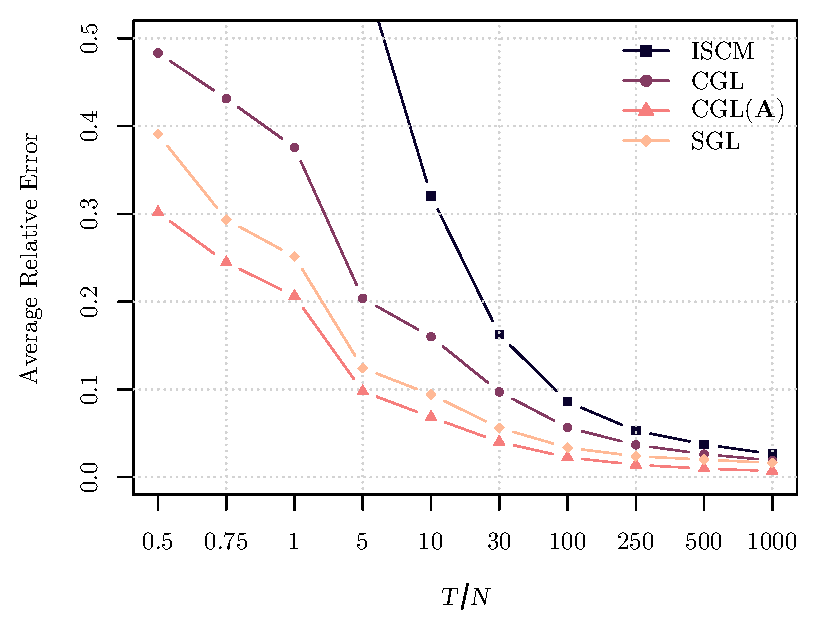
\includegraphics[width=\textwidth]{relative_error_grid.eps}
        \caption{Relative error versus $T/N$}
    \end{subfigure}
    ~ %add desired spacing between images, e. g. ~, \quad, \qquad, \hfill etc.
      %(or a blank line to force the subfigure onto a new line)
    \begin{subfigure}[b]{0.47\textwidth}
        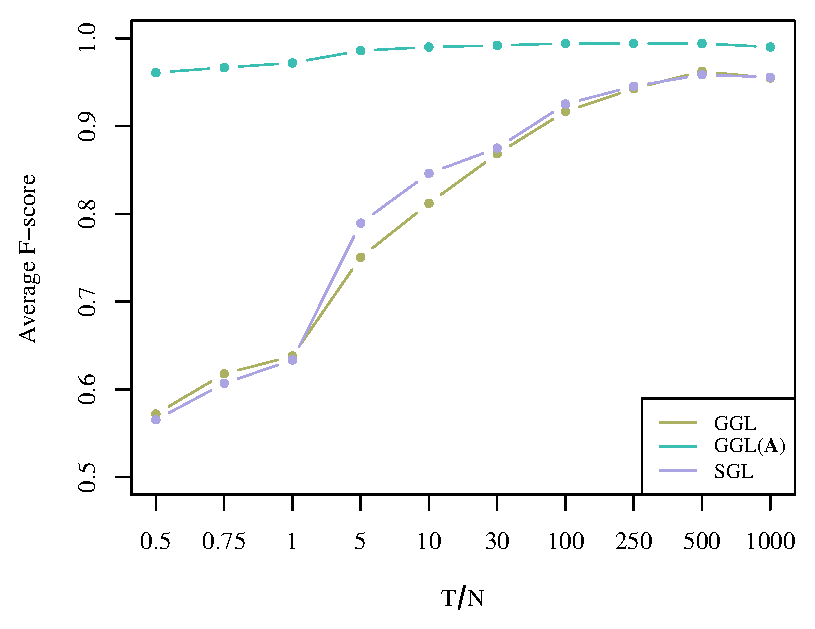
\includegraphics[width=\textwidth]{fscore_grid.eps}
        \caption{F-score versus $T/N$}
    \end{subfigure}
    \caption{Average performance results for learning Laplacian matrix of a $\mathcal{G}^{(64)}_{\mathsf{grid}}$.}
    \label{fig:performance}
\end{figure}

\end{document}
